\section{CalibX标定系统}
CalibX标定系统由软件系统和硬件系统组成。
\subsection{硬件}
硬件系统如图\ref{moon2_device}所示。该硬件系统主要由机械臂、标定板、光源、计算机及显示器、供电系统等组成。
\begin{figure}[h]
	\centering
	\includegraphics[width=1\textwidth]{figure/cp10/moon2_device}
	\caption{CalibX硬件系统}
	\label{moon2_device}
\end{figure}
该系统具有如下优点:
\begin{itemize}
	\item 立体标定板,支持大FOV鱼眼相机、支持多相机,多相机之间可以无重叠视场
	\item 4向可调高亮高均匀光源,箱体内镜头处光源强度可达2000lux,降低相机曝光时间,减轻卷帘曝光影响
	\item 机械臂、滑台滑环组合,连续转动不绕线
\end{itemize}
一些标定样品如图\ref{fig:calibx}所示。
\begin{figure}
	\centering
	\begin{minipage}{0.45\linewidth}
		\centering
		\subfigure[标定手机]{\includegraphics[width=\linewidth,height=8cm]{figure/cp10/cellphone}}
		\label{fig:subcaption1}
	\end{minipage}\qquad
	\begin{minipage}{0.45\linewidth}
		\centering
		\subfigure[标定眼镜]{\includegraphics[width=\linewidth,height=8cm]{figure/cp10/ar_glass}}
		\label{fig:subcaption2}
	\end{minipage}
	\caption{CalibX标定系统标定产品样例}
	\label{fig:calibx}
\end{figure}
\subsection{软件}
软件系统如图\ref{fig:calibx_framework}所示。整个标定系统主要包含四个模块:IMU噪声标定、静态相机标定、卷帘(rolling shutter,简称RS)RS标定和Visual-Inertial(VI)联标。
\begin{figure}[h]
	\centering
	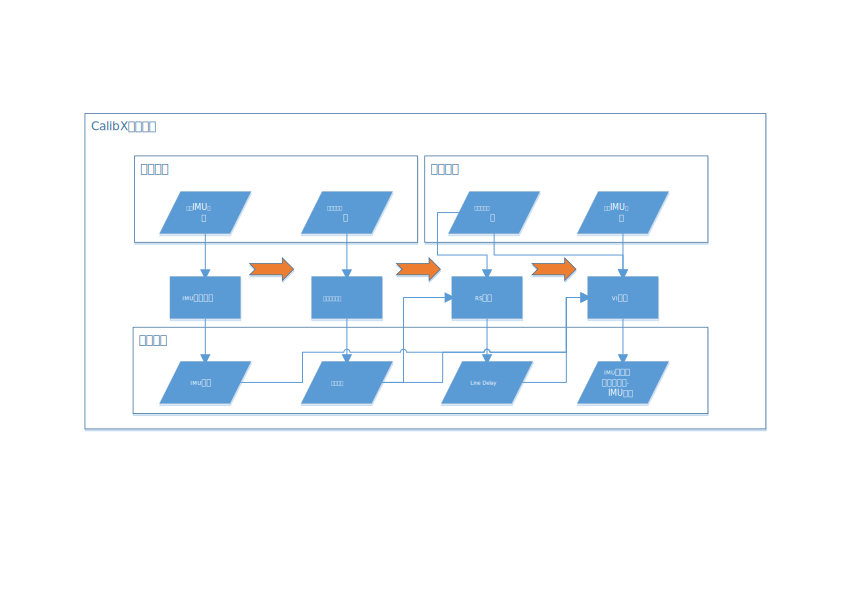
\includegraphics[width=1\textwidth]{figure/cp10/calibx_framework}
	\caption{CalibX硬件系统}
	\label{fig:calibx_framework}
\end{figure}
目前支持3种相机模型:
\begin{itemize}
	\item Pinhole-brown和pinhole-radtan。主要面向小畸变、小视场角(FOV)的相机。
	\item Pinhole-equidistant。主要面向大畸变、大视场角的相机(FOV $\le $ 180°),主要是广角相机和鱼眼相机。
\end{itemize}
支持4种标定板,如图\ref{fig:calibx-calibration-board}所示。:
\begin{itemize}
	\item 棋盘格。
	\item CircleGrid。
	\item Apriltag。
	\item RandomGrid。
\end{itemize}
\begin{figure}
	\centering
	\begin{minipage}{0.45\linewidth}
		\centering
		\subfigure[棋盘格]{\includegraphics[width=5cm]{figure/cp10/chessboard}}
		\label{fig:chessboard}
	\end{minipage}\qquad
	\begin{minipage}{0.45\linewidth}
		\centering
		\subfigure[CircleGrid]{\includegraphics[width=5cm]{figure/cp10/circlegrid}}
		\label{fig:circlegrid}
	\end{minipage}
	\begin{minipage}{0.45\linewidth}
		\centering
		\subfigure[Apriltag]{\includegraphics[width=5cm]{figure/cp10/apriltag}}
		\label{fig:apriltag}
	\end{minipage}\qquad
	\begin{minipage}{0.45\linewidth}
		\centering
		\subfigure[RandomGrid]{\includegraphics[width=5cm]{figure/cp10/randomgrid}}
		\label{fig:randomgrid}
	\end{minipage}
	\caption{CalibX标定系统支持的标定板}
	\label{fig:calibx-calibration-board}
\end{figure}
支持多标定板。